\documentclass[pdftex,12pt, oneside]{article}

%\usepackage[paperwidth=8.5in, paperheight=13in]{geometry} % Folio
\usepackage[paperwidth=8.27in, paperheight=11.69in]{geometry} % A4

\usepackage{makeidx}         % allows index generation
\usepackage{graphicx}        % standard LaTeX graphics tool
                             % when including figure files
\usepackage[bottom]{footmisc}% places footnotes at page bottom
\usepackage[english]{babel}
\usepackage{enumerate}
\usepackage{paralist}
\usepackage{float}
\usepackage{gensymb}  
\usepackage{listings}
\usepackage{color}
\usepackage{mathtools} % atau \usepackage{amsmath}
\renewcommand{\baselinestretch}{1.5}

\newcommand{\HRule}{\rule{\linewidth}{0.5mm}}

\definecolor{codegreen}{rgb}{0,0.6,0}
\definecolor{codegray}{rgb}{0.5,0.5,0.5}
\definecolor{codepurple}{rgb}{0.58,0,0.82}
\definecolor{backcolor}{rgb}{0.95,0.95,0.92}

\lstdefinestyle{mystyle}{
  backgroundcolor=\color{backcolor},
  commentstyle=\color{codegreen},
  keywordstyle=\color{magenta},
  stringstyle=\color{codepurple},
  basicstyle=\footnotesize,
  breakatwhitespace=false,
  breaklines=true,
  captionpos=b,
  keepspaces=true,
  numbers=left,
  numbersep=5pt,
  showspaces=false,
  showstringspaces=false,
  showtabs=false,
  tabsize=2
}

\lstset{style=mystyle}


\begin{document}
\sloppy % biar section ga melebar melewati kertas

\begin{center}
{\large RANCANGAN RINCI SISTEM \textit{WEB SERVICES} SEBAGAI CARA KOMUNIKASI DENGAN TEMPAT PEMBAYARAN DALAM PENCATATAN PEMBAYARAN PAJAK BUMI DAN BANGUNAN PERDESAAN DAN PERKOTAAN DI KABUPATEN BREBES.}
\\[1cm]
DD MMM 2016\\
Priyanto Tamami, S.Kom.
\end{center}

%\frontmatter%%%%%%%%%%%%%%%%%%%%%%%%%%%%%%%%%%%%%%%%%%%%%%%%%%%%%%


%%%%%%%%%%%%%%%%%%%%%%%%%%%%%%%%%%%%%%%%%%%%%%%%%%%%%%%%%%%%%%%%%%%%%%

\section{SISTEM KOMPUTER}

Sistem komputer yang digunakan akan terbagi menjadi 3 (tiga) yaitu :

\begin{enumerate}[1.]
  \item Sebagai \textit{server} basis data adalah sebagai berikut :

    \begin{itemize}
      \item Prosesor Intel Xeon 2,4GHz
      \item Memori 44GB
      \item Sistem Operasi Windows Server 2008 R2 64 bit.
    \end{itemize}
    
  \item Sebagai \textit{server} aplikasi adalah sebagai berikut :
  
    \begin{itemize}
      \item Prosesor Intel Xeon 3,1GHz
      \item Memori 4GB
      \item Sistem Operasi CentOS 6.2 64 bit
    \end{itemize}
    
  \item Sebagai \textit{client} spesifikasi yang digunakan bebas, dapat menggunakan sistem komputer apapun yang dapat berkomunikasi melalui jaringan TCP/IP.
  
  Karena \textit{client} nantinya adalah Bank sebagai tempat pembayaran, maka sebagai sarana untuk uji coba dapat menggunakan sistem komputer apapun dengan \textit{browser} Chrome / Firefox.

\end{enumerate}

\section{SISTEM JARINGAN}

Sistem jaringan yang nantinya dibangun akan terlihat seperti pada gambar \ref{fig:network-diagram} :

\begin{figure}[H]
  \centering
  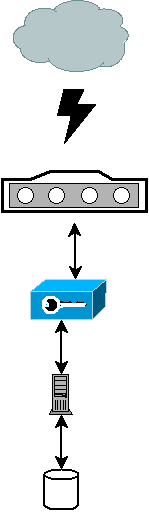
\includegraphics[width=0.2\textwidth]{./resources/diagram/network-diagram}
  \caption{Diagram Sistem Jaringan \textit{Web Services} PBB}
  \label{fig:network-diagram}
\end{figure}

Dari diagram tersebut, gambar awan adalah simbol untuk jaringan internet. Untuk melakukan akses ke \textit{server web service} akan melalui modem dibawahnya, kemudian akan menghubungi VPN \textit{server} terlebih dahulu untuk mendapatkan otentikasi atau akses ke dalam jaringan internal.

Setelah sukses melakukan otentikasi ke \textit{server} VPN, selanjutnya \textit{client} dalam hal ini Bank akan melakukan akses ke \textit{server web service} langsung, dimana \textit{server web service} akan melakukan komunikasi dengan \textit{server} basis data.

\section{SISTEM BASIS DATA}

Sistem basis data yang digunakan adalah sama dengan sistem basis data yang digunakan pada SISMIOP untuk pengelolaan PBB-P2, yaitu sistem basis data Oracle Database 11g. Namun tidak semua objek digunakan pada sistem \textit{web service} yang akan dibangun. Beberapa tabel yang digunakan adalah sebagai berikut :

\begin{itemize}
  \item Tabel SPPT
  
  Tabel SPPT ini nantinya hanya akan merubah pada kolom STATUS\_PEMBAYARAN\_SPPT, untuk isian 0 (nol) artinya nomor objek pajak (NOP) untuk tahun pajak tersebut belum dibayarkan, sedangkan isian 1 (satu) artinya NOP untuk tahun pajak tersebut sudah terbayar.
  
  \item Tabel PEMBAYARAN\_SPPT
  
  Tabel PEMBAYARAN\_SPPT ini apabila ada transaksi pembayaran, akan dicatatkan lengkap pada tabel ini, NOP apa, tahun pajak kapan, besarnya nilai yang dibayarkan, tanggal pembayaran, semuanya tersimpan pada tabel ini. Namun bila terjadi permintaan proses \textit{reversal}, maka data yang tersimpan pada tabel ini akan dihapuskan.
  
  \item Tabel LOG\_TRX\_PEMBAYARAN
  
  Tabel LOG\_TRX\_PEMBAYARAN ini digunakan untuk menyimpan aktivitas transaksi pembayaran yang sukses.
  
  \item Tabel LOG\_REVERSAL
  
  Tabel LOG\_REVERSAL digunakan untuk menyimpan aktivitas \textit{reversal} yang berhasil dilakukan pada basis data.
\end{itemize}

Beberapa \textit{store procedure} juga dibuat untuk mempercepat eksekusi proses, \textit{store procedure} ini, \textit{store procedure} yang dibuat adalah sebagai berikut :

\begin{itemize}
  \item SPPT\_TERHUTANG
  
  \textit{Store procedure} ini akan bertugas memberikan data SPPT terhutang ke aplikasi yang melakukan eksekusi terhadapnya.
  
  \item PROSES\_PEMBAYARAN
  
  \textit{Store procedure} ini akan bertugas melakukan pencatatan pembayaran pada tabel PEMBAYARAN\_SPPT, melakukan perubahan isi kolom STATUS\_PEMBAYARAN\_SPPT pada tabel SPPT, kemudian melakukan pencatatan prosesnya pada tabel LOG\_TRX\_PEMBAYARAN.
  
  \item REVERSAL\_PEMBAYARAN
  
  \textit{Store procedure} ini bertugas melakukan penghapusan data pada tabel PEMBAYARAN\_SPPT, merubah kolom STATUS\_PEMBAYARAN\_SPPT pada tabel SPPT menjadi 0 (nol), dan melakukan pencatatan pada tabel LOG\_REVERSAL.
\end{itemize}

\section{PROSEDUR AKTIVITAS}

Prosedur aktivitas yang berlaku untuk sistem \textit{web services} ini akan terbagi menjadi beberapa skenario yang dituangkan dalam beberapa diagram untuk mempermudah pemahaman alur aktivitas yang terjadi. Berikut adalah diagram yang terbentuk.

\subsection{Diagram \textit{Use-Case}}

Pembahasan skenario utama terdapat pada diagram \textit{use-case} seperti pada gambar \ref{fig:uml-use-case} :

\begin{figure}[H]
  \centering
  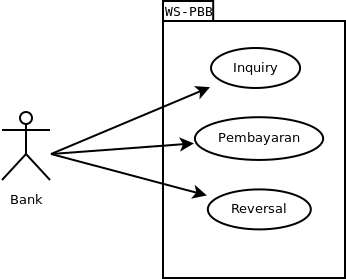
\includegraphics[width=0.5\textwidth]{./resources/diagram/uml-use-case}
  \caption{Diagram \textit{Use-Case}}
  \label{fig:uml-use-case}
\end{figure}

Seperti terlihat pada diagram, skenario utama atau fitur dari \textit{web service} PBB-P2 akan melayani \textit{inquiry}, transaksi pembayaran, dan \textit{reversal} pembayaran.

Secara mendalam, tiap skenario utama nantinya akan terbagi menjadi beberapa skenario rinci yang dijelaskan dalam beberapa diagram berbeda.

\subsection{Diagram \textit{Activity}}

Dari 3 (tiga) skenario utama, akan muncul aktivitas detail yang digambarkan oleh diagram \textit{activity} berikut :

\subsubsection{Diagram \textit{Activity Inquiry}}

Pada diagram untuk skenario ini akan menjelaskan gambaran aktivitas \textit{inquiry} yang terjadi dan bagaiamana respon terhadap \textit{request inquiry} diselesaikan. Diagramnya seperti terlihat pada gambar \ref{fig:uml-act-inq} :

\begin{figure}[H]
  \centering
  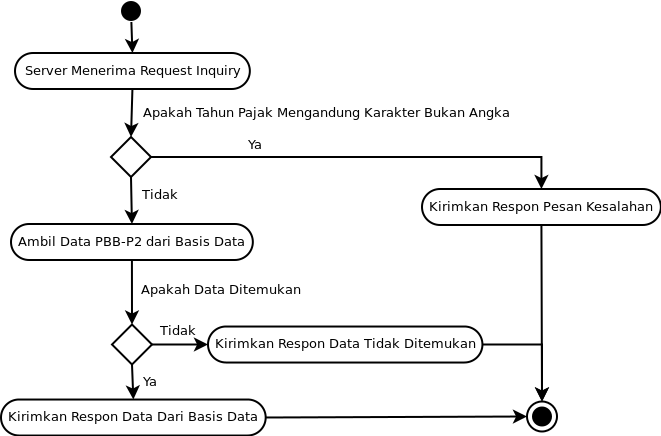
\includegraphics[width=0.7\textwidth]{./resources/diagram/uml-act-inquiry}
  \caption{Diagram \textit{Activity Inquiry}}
  \label{fig:uml-act-inq}
\end{figure}

Skenario ini diawali dari \textit{server} yang menerima \textit{request inquiry} dari \textit{client}, kemudian \textit{server} melakukan pemeriksaan pada parameter tahun pajak yang diberikan, apakah mengandung karakter bukan angka atau merupakan karakter angka seluruhnya. Bila parameter tahun pajak mengandung karakter bukan angka, maka \textit{server} akan mengirimkan respon pesan kesalahan ke \textit{client}. Namun bila berhasil, maka melanjutkan ke aktivitas berikutnya yaitu mengambil data PBB-P2 pada basis data.

Hasil dari pengambilan data PBB-P2 pada basis data ada 2 (dua) kemungkinan, yaitu data ditemukan, dan data tidak ditemukan pada basis data.

Bila data tidak ditemukan pada basis data, maka \textit{server} akan mengirimkan respon pesan bahwa data yang diminta tidak ditemukan dalam basis data, sedangkan bila data ditemukan, maka \textit{server} akan memberikan respon pesan berupa data-data yang dibutuhkan dari basis data.

\subsubsection{Diagram \textit{Activity} Pencatatan Pembayaran}

Diagram ini akan menjelaskan aktivitas yang terjadi pada saat \textit{request} pencatatan pembayaran diterima oleh \textit{server}, bentuk diagramnya akan terlihat seperti pada gambar \ref{fig:uml-act-bayar} :

\begin{figure}[H]
  \centering
  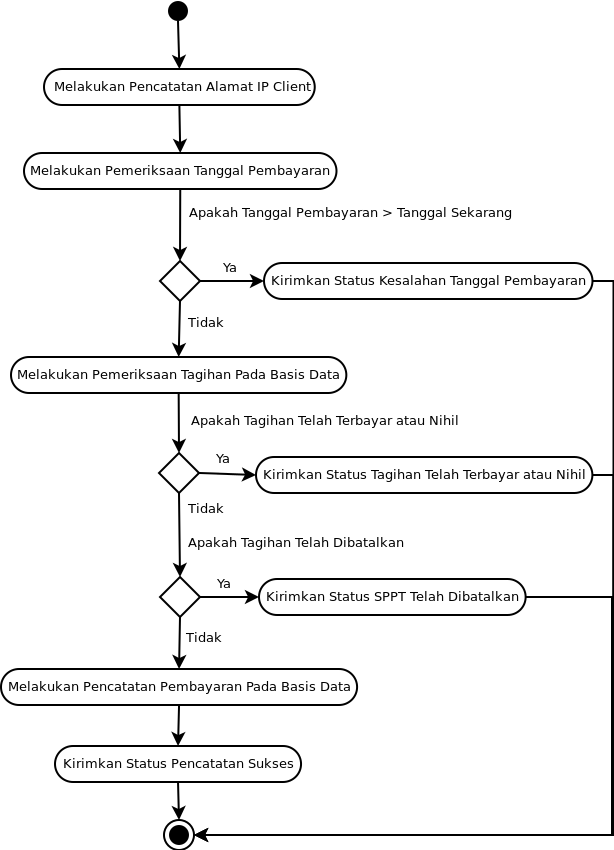
\includegraphics[width=0.8\textwidth]{./resources/diagram/uml-act-bayar}
  \caption{Diagram \textit{Activity} Pencatatan Pembayaran}
  \label{fig:uml-act-bayar}
\end{figure}

Bila ada \textit{request} pencatatan pembayaran, langkah yang pertama adalah melakukan pencatatan alamat IP \textit{client}, kemudian melakukan pemeriksaan parameter tanggal pembayaran yang diberikan \textit{client}, apakah tanggal pembayaran terjadi setelah tanggal dan jam saat ini, atau sebelum tanggal dan jam saat ini.

Bila tanggal dan jam pembayaran melewati tanggal dan jam saat ini, maka \textit{server} akan mengirimkan status kesalahan tanggal pembayaran dan proses selesai sampai disini.

Ketika tanggal dan jam pembayaran sebelum tanggal dan jam saat ini, proses dilanjutkan dengan melakukan pemeriksaan tagihan pada basis data. Bila tagihan untuk data yang diminta berdasarkan Nomor Objek Pajak (NOP) dan tahun pajak telah terbayar atau nihil pada basis data, maka \textit{server} akan mengirimkan status bahwa tagihan tersebut telah terbayar atau tagihan nihil kepada \textit{client} dan proses selesai sampai disini.

Pemeriksaan pun dilanjutkan apakah NOP untuk tahun pajak tersebut telah dibatalkan atau tidak. Bila telah dibatalkan maka \textit{server} akan mengirimkan status bahwa tagihan atas NOP untuk tahun pajak tersebut telah dibatalkan.

Bila seleksi atau pemeriksaan atas NOP untuk tahun pajak yang diminta muncul tagihan dan belum terbayar, status tagihannya pun tidak dibatalkan, maka \textit{server} melakukan pencatatan pembayaran pada basis data, dan mengirimkan status sukses ke \textit{client} sebagai sinyal bahwa \textit{request} pencatatan pembayaran telah berhasil dilakukan. Sampai sini proses pencatatan pembayaran selesai.

\subsubsection{Diagram \textit{Activity Reversal}}

Diagram ini akan menjelaskan aktivitas yang terjadi apabila ternyata ada kesalahan pencatatan pembayaran, sehingga aktivitas pencatatan pembayaran yang telah terjadi harus dikembalikan pada kondisi semula. Diagram aktivitas ini adalah seperti pada gambar \ref{fig:uml-act-reversal} : 

\begin{figure}[H]
  \centering
  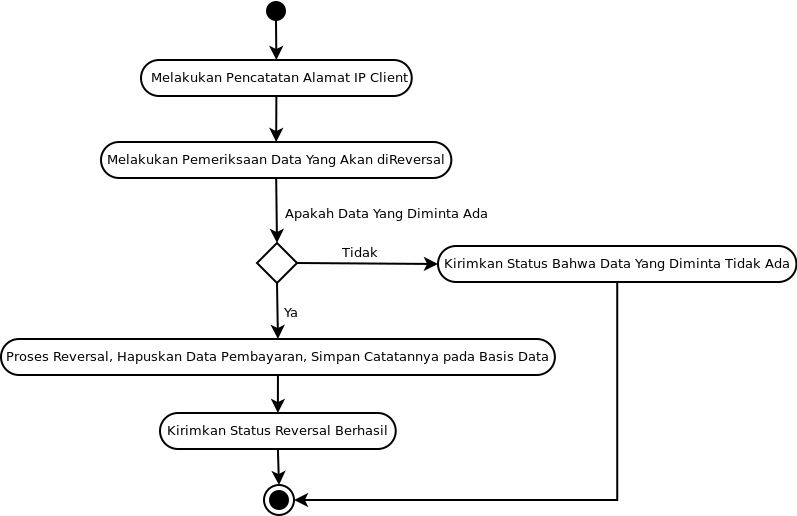
\includegraphics[width=0.8\textwidth]{./resources/diagram/uml-act-reversal}
  \caption{Diagram \textit{Activity} Untuk \textit{Reversal} Pencatatan Pembayaran}
  \label{fig:uml-act-reversal}
\end{figure}

Setiap ada \textit{request reversal} yang diterima, maka \textit{server} akan melakukan pencatatan alamat IP \textit{client}, kemudian akan dilakukan pemeriksaan data yang akan dilakukan \textit{reversal}, apakah data yang diinginkan ada pada basis data atau tidak.

Bila data tidak ditemukan pada basis data, maka \textit{server} akan mengirimkan status ke \textit{client} bahwa data yang diminta untuk dilakukan \textit{reversal} tidak ada pada basis data.

Bila data ditemukan pada basis data, maka \textit{server} akan melakukan proses \textit{reversal} dengan cara menghapus data pembayaran, dan melakukan pencatatan aktivitas \textit{reversal} pada tabel terpisah, terakhir adalah mengirimkan status ke \textit{client} bahwa proses \textit{reversal} yang diminta telah berhasil dilakukan.

\subsection{Diagram \textit{Entity Relational}}

Diagram ini akan memperlihatkan struktur tabel dan hubungan antar tabel yang digunakan pada sistem aplikasi \textit{web services} PBB-P2. Diagramnya seperti terlihat pada gambar \ref{fig:uml-entity-relational} :

\begin{figure}[H]
  \centering
  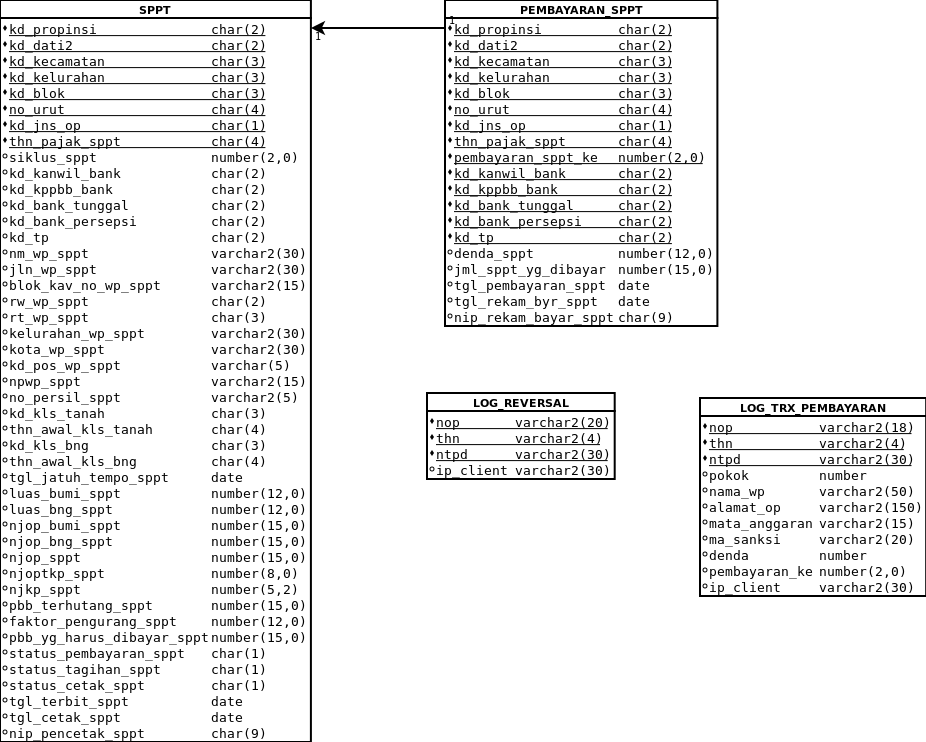
\includegraphics[width=1\textwidth]{./resources/diagram/uml-entity-relational}
  \caption{Diagram \textit{Entity Relational}}
  \label{fig:uml-entity-relational}
\end{figure}

Pada tabel SPPT akan berisi seluruh tagihan PBB-P2 untuk seluruh tahun pajak. Tabel ini akan menjadi induk atau acuan dari tabel-tabel yang nantinya digunakan pada sistem ini. Namun kondisi yang nantinya berubah karena interaksi sistem \textit{web service} dengan basis data dari tabel SPPT ini hanya pada kolom STATUS\_PEMBAYARAN\_SPPT.

Tabel yang kedua adalah tabel PEMBAYARAN\_SPPT, yang menjadi tempat tampungan data dari transaksi pembayaran. Seluruh penerimaan / pembayaran PBB-P2 yang terjadi harus tercatat pada tabel ini. Kolom KD\_PROPINSI, KD\_DATI2, KD\_KECAMATAN, KD\_KELURAHAN, KD\_BLOK, NO\_URUT, KD\_JNS\_OP, dan THN\_PAJAK\_SPPT akan mengacu pada tabel SPPT.

Tabel ketiga adalah tabel LOG\_TRX\_PEMBAYARAN, tabel ini berfungsi untuk melakukan pencatatan aktivitas sistem, setelah melakukan perubahan pada kolom STATUS\_PEMBAYARAN\_SPPT milik tabel SPPT dari 0 (nol) menjadi 1 (satu), dan setelah melakukan pengisian data pada tabel PEMBAYARAN\_SPPT, maka dicatatkan pula informasi aktivitasnya pada tabel LOG\_TRX\_PEMBAYARAN.

Tabel berikutnya adalah tabel LOG\_REVERSAL, tabel ini berfungsi untuk mencatat aktivitas \textit{reversal} yang terjadi, setelah kondisi kolom STATUS\_PEMBAYARAN\_SPPT pada tabel SPPT berubah dari 1 (satu) menjadi 0 (nol, dan setelah penghapusan data pada tabel PEMBAYARAN\_SPPT.

\subsection{Diagram \textit{Class}}

Diagram ini akan memperlihatkan kelas atau objek apa saja yang terbentuk untuk membangun sistem \textit{web service} ini dapat bekerja sebagaimana mestinya, diagram \textit{class} adalah sebagaimana gambar \ref{fig:uml-class} :

\begin{figure}[H]
  \centering
  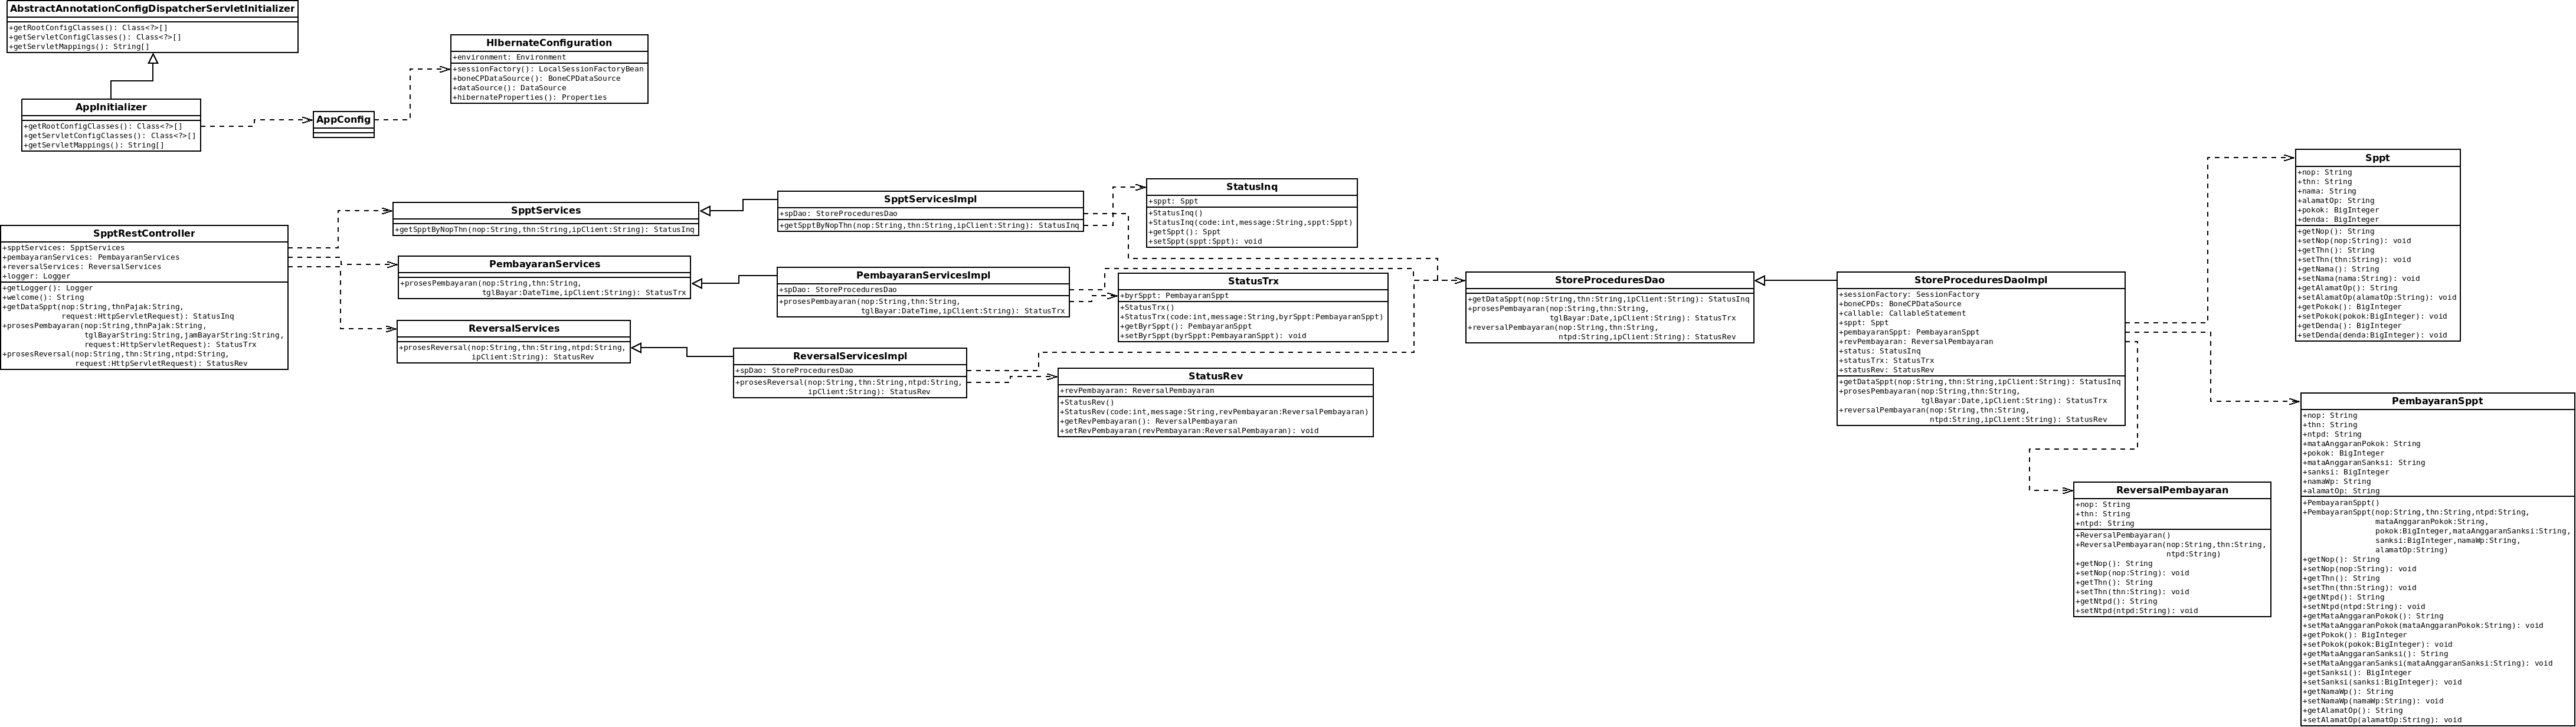
\includegraphics[width=1\textwidth]{./resources/diagram/uml-class}
  \caption{Diagram \textit{Class}}
  \label{fig:uml-class}
\end{figure}

kelas-kelas tersebut akan dijelaskan sebagai berikut :

\begin{enumerate}[1.]
  \item \textit{Interface} AbstractAnnotationConfigDispatcherServletInitializer
  
  \textit{Interface} ini sebetulnya bawaan dari \textit{framework} Spring yang digunakan untuk melakukan inisialisasi parameter awal dari sistem yang akan digunakan. Artinya setiap kelas yang melakukan \textit{implement} terhadap \textit{interface} ini nantinya akan digunakan sebagai pintu masuk awal sistem melakukan pengaturan-pengaturan / inisialisasi.
  
  \item Kelas AppInitializer
  
  Kelas inilah yang mengimplementasikan \textit{interface} AbstractAnnotationConfigDispatcherServletInitializer, sehingga dari kelas inilah sistem akan memulai aktivitasnya.
  
  \item Kelas AppConfig
  
  Kelas ini digunakan sebagai tempat untuk konfigurasi sistem \textit{web service} yang nantinya berjalan. Setelah sistem melakukan inisialisasi awal di kelas AppInitializer, kelas AppConfig ini nantinya melakukan konfigurasi kelas-kelas mana yang akan berhubungan dengan basis data, kelas mana yang nantinya melakukan konfigurasi hubungan antar kelas dan cara interaksinya.
  
  \item Kelas HibernateConfiguration
  
  Kelas ini nantinya menjadi tempat konfigurasi \textit{framework} Hibernate sebagai penghubung antara sistem aplikasi dengan basis data.
  
  \item Kelas SpptRestController
  
  Kelas ini adalah tempatnya sistem aplikasi berhubungan dengan \textit{client}. Setiap \textit{request} yang dikirim oleh \textit{client} akan masuk melalui kelas ini.
  
  \item \textit{Interface} SpptServices
  
  \textit{Interface} ini nantinya akan menyiapkan beberapa \textit{method} yang akan diimplementasikan di kelas turunannya, sehingga kelas turunan dapat mengolah dan menyajikan berbagai data yang berhubungan dengan informasi SPPT. \textit{Interface} ini pula yang nantinya menghubungkan kelas SpptRestController dengan beberapa \textit{service} yang dibutuhkan dan berhubungan dengan SPPT.
  
  \item \textit{Interface} PembayaranServices
  
  \textit{Interface} ini seperti \textit{interface} SpptServices, yaitu menyiapkan \textit{method} yang akan diimplementasikan di kelas turunan yang dapat mengolah dan menyajikan atau memproses data yang berhubungan dengan proses pencatatan pembayaran.
  
  \item \textit{Interface} ReversalServices
  
  Sebagaimana \textit{interface} SpptServices dan PembayaranServices, \textit{interface} ini pun hanya menyiapkan \textit{method} yang akan diimplementasikan di kelas turunan yang berhubungan dengan kegiatan \textit{reversal} pembayaran.
  
  \item Kelas SpptServicesImpl
  
  Kelas ini adalah implementasi dari \textit{interface} SpptServices yang akan mengolah dan menyajikan data terkait dengan \textit{request inquiry} data SPPT. 
  
  \item Kelas PembayaranServicesImpl
  
  Kelas ini adalah implementasi dari \textit{interface} PembayaranServices yang akan mengolah dan menyajikan data terkait dengan proses pencatatan pembayaran PBB-P2.
  
  \item Kelas ReversalServicesImpl
  
  Kelas ini adalah implementasi dari \textit{interface} ReversalServices yang akan mengolah dan menyajikan data terkait dengan proses \textit{reversal} pembayaran PBB-P2.
  
  \item Kelas StatusInq
  
  Kelas ini akan menampung informasi untuk proses \textit{inquiry}, nantinya dari kelas ini akan secara otomatis menggunakan pustaka Jackson diubah ke format JSON sebagai bentuk komunikasi ke \textit{client}.
  
  \item Kelas StatusTrx
  
  Kelas ini akan menampung informasi yang dihasilkan dari aktivitas pencatatan transaksi pembayaran, kelas ini pun nantinya akan diubah otomatis oleh pustaka Jackson ke bentuk JSON sebagai format komunikasi dengan \textit{client}.
  
  \item Kelas StatusRev
  
  Kelas ini akan menampung informasi yang dihasilkan dari proses \textit{reversal} pembayaran, kelas ini juga akan diubah secara otomatis ke bentuk JSON oleh pustaka Jackson sebagai format baku komunikasi dengan \textit{client}.
  
  \item \textit{Interface} StoreProceduresDao
  
  \textit{Interface} ini akan menyiapkan \textit{method} yang digunakan oleh kelas turunan sebagai bahan untuk berkomunikasi dengan basis data. Tujuan lain dari pembentukan \textit{interface} ini pun untuk mempermudah \textit{framework} melakukan pemetaan mana kelas yang nantinya akan berhubungan dengan basis data.
  
  \item Kelas StoreProceduresDaoImpl
  
  Kelas ini adalah implementasi dari \textit{interface} StoreProceduresDao, nantinya setiap eksekusi \textit{store procedure} milik basis data akan dilakukan dari kelas ini. Dari kelas ini pun hasilnya nanti didapat dan dikembalikan ke \textit{client}.
  
  \item Kelas Sppt
  
  Kelas ini nantinya akan menampung hasil dari pemanggilan \textit{store procedure} milik basis data untuk aktivitas \textit{inquiry} data PBB-P2.
  
  \item Kelas PembayaranSppt
  
  Kelas ini akan menampung hasil dari pemanggilan \textit{store procedure} milik basis data untuk proses pencatatan pembayaran PBB-P2.
  
  \item Kelas ReversalPembayaran
  
  Kelas ini akan menampung hasil dari pemanggilan \textit{store procedure} milik basis data untuk proses \textit{reversal} pembayaran PBB-P2.
  
\end{enumerate}

\subsection{Diagram \textit{Sequence}}

Diagram \textit{sequence} akan menggambarkan interaksi antar kelas berdasarkan skenario-skenario yang telah disusun sehingga sistem aplikasi \textit{web service} nantinya akan berjalan sebagaimana mestinya. Adapun skenario-skenario tersebut akan dibagi seperti berikut ini :

\subsubsection{Skenario Konfigurasi \textit{Spring Framework}}
\subsubsection{Skenario \textit{Inquiry} Gagal Karena Tahun Pajak Bukan Angka}
\subsubsection{Skenario \textit{Inquiry} Gagal Karena Data Tidak Ditemukan}
\subsubsection{Skenario \textit{Inquiry} Gagal Karena Kesalahan \textit{Server}}
\subsubsection{Skenario \textit{Inquiry} Yang Sukses}
\subsubsection{Skenario Transaksi Pembayaran Gagal Karena Jam Pembayaran Melebihi Jam Pencatatan}
\subsubsection{Skenario Transaksi Pembayaran Gagal Karena Tagihan Telah Terbayar atau Nihil}
\subsubsection{Skenario Transaksi Pembayaran Gagal Karena Telah Dibatalkan}
\subsubsection{Skenario Transaksi Pembayaran Gagal Karena Kesalahan \textit{Server}}
\subsubsection{Skenario Transaksi Pembayaran Yang Sukses}
\subsubsection{Skenario \textit{Reversal} Gagal Karena Data Yang Diminta Tidak Ada}
\subsubsection{Skenario \textit{Reversal} Gagal Karena Ada Data Pembayaran Yang Tercatat Ganda}
\subsubsection{Skenario \textit{Reversal} Gagal Karena Kesalahan \textit{Server}}
\subsubsection{Skenario \textit{Reversal} Yang Sukses}

\subsection{Diagram \textit{Deployment}}

\section{SUMBER DAYA MANUSIA}

Karena bentuk sistem ini adalah bentuk otomasi dari pencatatan pembayaran, dimana komunikasi yang terjadi antara \textit{server} pada DPPK Kabupaten Brebes dengan \textit{server} pada Bank sebagai tempat pembayaran, tidak ada sumber daya manusia yang berinteraksi secara langsung dengan sistem ini.

\end{document}